\section{Experiment}
\label{sec:exp}

\subsection{Experimental Setup}

\subsubsection{Datasets}
\label{sec:setup_data}
We evaluate our approach on three representative driving benchmarks. 
For all datasets, the router is trained on static detection images and tested on continuous video sequences, without any temporal or tracking supervision at any stage.
We assume no significant train-deployment distribution shift; the primary difference lies in the temporal structure of the deployment videos.

\noindent\textbf{KITTI.} 
We train the router on the KITTI Detection dataset~\cite{geiger2012kitti} using an 80:20 split of 5,985 training and 1,496 validation images, and evaluate it on the KITTI Multi-Object Tracking benchmark consisting of 21 video sequences (8,008 frames). 
Frames are processed at a resolution of $384\times1248$.

\noindent\textbf{BDD100K.} 
To evaluate cross-dataset generalization, we train the router on BDD100K detection images~\cite{yu2020bdd} (70K train, 10K val) and evaluate on the BDD100K MOT validation split comprising 200 video sequences. 
Frames are processed at $720\times1280$ resolution.

\noindent\textbf{Waymo.}
To further evaluate generalization on a large-scale, high-resolution benchmark, we use the front camera of the Waymo Open Perception dataset~\cite{sun2020waymo} (v2.0.1). 
As this benchmark provides no separate detection and tracking splits, we partition it by official split: the router is trained on the 798 training-split segments treated as static detection images (158.1K frames), and evaluated on the 202 validation-split segments as continuous video (39.1K labeled frames).
Frames are processed at $1280\times1920$ resolution.
% Consequently, unlike KITTI and BDD100K---where the image-level router analysis and the final video evaluation use distinct detection and tracking sets---both the image-level calibration (Sec.~\ref{sec:results_calibration}) and the video evaluation here are performed on the same validation split; the training split remains fully disjoint, so no router ever observes its evaluation data.
% Following the official Waymo 2D camera-image detection task, AP is computed (with 2D IoU matching) over the \texttt{vehicle}, \texttt{pedestrian}, and \texttt{cyclist} classes.


% NOTE: Figure 5 and Table 3 both report DIRECTLY-MEASURED operating points --
% each is the router run on the streaming video at a fixed tau (no interpolation).
% An alternative unified-grid {0,...,100}% version of Table 3 (tau/AP interpolated
% along the measured curve) is preserved, commented, at the end of the tab:main block.
\begin{figure*}[!t]
\centering
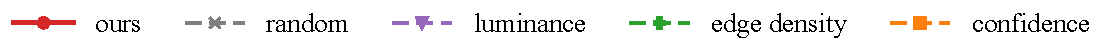
\includegraphics[width=0.86\textwidth]{fig_main_legend.pdf}\\[2pt]
\begin{minipage}[t]{0.32\textwidth}
\centering
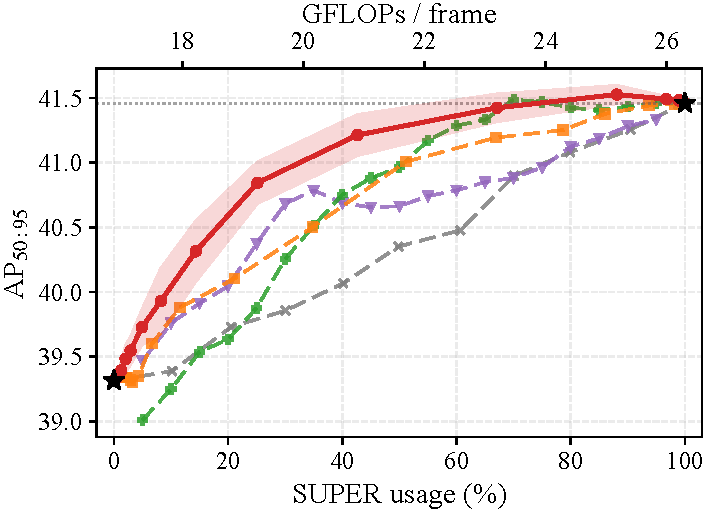
\includegraphics[width=\linewidth]{fig_main_kitti_ap5095.pdf}
\vspace{2pt}
{\small (a) KITTI}
\end{minipage}\hfill
\begin{minipage}[t]{0.32\textwidth}
\centering
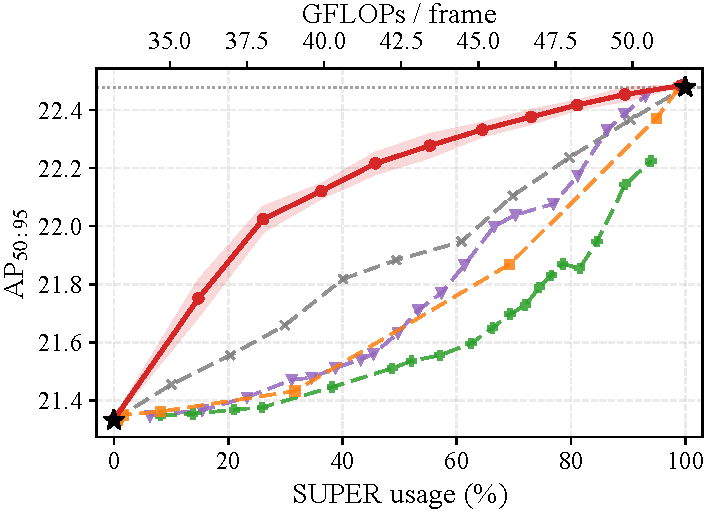
\includegraphics[width=\linewidth]{fig_main_bdd_ap5095.pdf}
\vspace{2pt}
{\small (b) BDD100K}
\end{minipage}\hfill
\begin{minipage}[t]{0.32\textwidth}
\centering
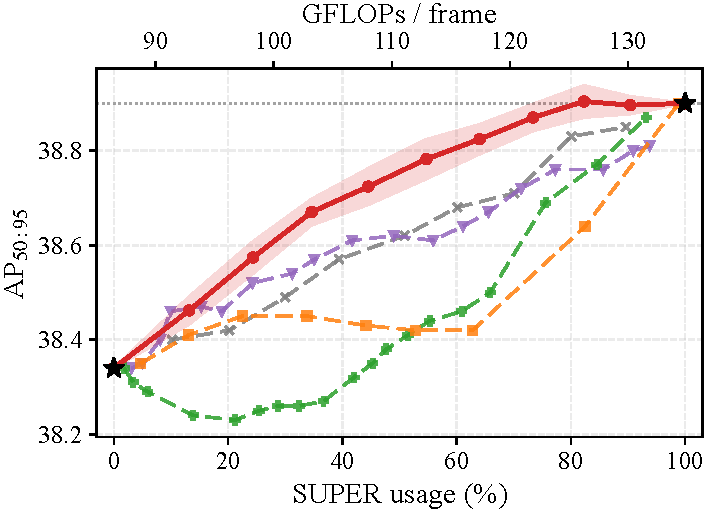
\includegraphics[width=\linewidth]{fig_main_waymo_ap5095.pdf}
\vspace{2pt}
{\small (c) Waymo}
\end{minipage}
\caption{
    Pareto-front evaluation of depth routing on (a) KITTI-Tracking, (b) BDD100K MOT, and (c) Waymo Open.
    Each point on the proposed curve corresponds to a different routing threshold $\tau$.
    We compare the advantage-regression router against random, luminance-, edge-density-, and confidence-based routing baselines in terms of AP@[.50:.95] versus SUPER-path usage.
    A single trained router traces a continuous accuracy--efficiency Pareto frontier that consistently dominates all baselines across all three benchmarks, with the largest gains observed in the low-compute regime where SUPER-path execution is limited.
}
\label{fig:main}
\end{figure*}


\begin{table*}[!t]
\caption{
    Efficiency of threshold-based depth routing across the operating points in Figure~\ref{fig:main}.
    AP denotes AP@[.50:.95] (\%).
    Latency, FPS, and energy are measured on a Jetson Orin Nano (TensorRT FP16) and include router overhead.
    always-super and always-base represent the static single-path baselines corresponding to the two endpoints of the Pareto frontier.
}
\label{tab:main}
\small
\setlength{\tabcolsep}{2.5pt}
\centering
\begin{minipage}[t]{0.49\textwidth}
\centering
{\small (a) KITTI}\\[2pt]
\footnotesize
\begin{tabular}{lrrrrrr}
\toprule
$\tau$ & SUPER\% & GFLOPs & AP & Latency (ms) & FPS & Energy (mJ)\\
\midrule
\textsc{always-base} & 0 & 16.87 & 39.3 & 12.99 & 77.0 & 248\\
$+0.70$ & 2.9 & 17.14 & 39.5 & 13.23 & 75.6 & 253\\
$+0.50$ & 8.2 & 17.64 & 39.9 & 13.66 & 73.2 & 261\\
$+0.40$ & 14.3 & 18.22 & 40.3 & 14.17 & 70.6 & 271\\
$+0.30$ & 25.1 & 19.24 & 40.8 & 15.06 & 66.4 & 289\\
$+0.20$ & 42.7 & 20.89 & 41.2 & 16.50 & 60.6 & 317\\
$+0.10$ & 67.1 & 23.20 & 41.4 & 18.51 & 54.0 & 357\\
$+0.00$ & 88.1 & 25.18 & 41.5 & 20.24 & 49.4 & 391\\
$-0.10$ & 96.7 & 25.99 & 41.5 & 20.95 & 47.7 & 405\\
$-0.40$ & 99.6 & 26.27 & 41.5 & 21.19 & 47.2 & 410\\
\textsc{always-super} & 100 & 26.30 & 41.5 & 21.22 & 47.1 & 410\\
\bottomrule
\end{tabular}
\end{minipage}\hfill
\begin{minipage}[t]{0.49\textwidth}
\centering
{\small (b) BDD100K}\\[2pt]
\footnotesize
\begin{tabular}{lrrrrrr}
\toprule
$\tau$ & SUPER\% & GFLOPs & AP & Latency (ms) & FPS & Energy (mJ)\\
\midrule
\textsc{always-base} & 0 & 33.18 & 21.3 & 25.08 & 39.9 & 520\\
$+0.086$ & 14.8 & 35.92 & 21.8 & 27.55 & 36.3 & 572\\
$+0.072$ & 26.1 & 38.02 & 22.0 & 29.43 & 34.0 & 613\\
$+0.064$ & 36.3 & 39.91 & 22.1 & 31.13 & 32.1 & 649\\
$+0.058$ & 45.8 & 41.66 & 22.2 & 32.71 & 30.6 & 683\\
$+0.054$ & 55.3 & 43.43 & 22.3 & 34.30 & 29.2 & 717\\
$+0.049$ & 64.5 & 45.14 & 22.3 & 35.83 & 27.9 & 750\\
$+0.045$ & 73.0 & 46.72 & 22.4 & 37.25 & 26.8 & 780\\
$+0.040$ & 81.1 & 48.21 & 22.4 & 38.60 & 25.9 & 809\\
$+0.033$ & 89.4 & 49.76 & 22.5 & 39.98 & 25.0 & 839\\
\textsc{always-super} & 100 & 51.72 & 22.5 & 41.75 & 24.0 & 877\\
\bottomrule
\end{tabular}
\end{minipage}

\vspace{8pt}

\begin{minipage}[t]{0.49\textwidth}
\centering
{\small (c) Waymo}\\[2pt]
\footnotesize
\begin{tabular}{lrrrrrr}
\toprule
$\tau$ & SUPER\% & GFLOPs & AP & Latency (ms) & FPS & Energy (mJ)\\
\midrule
\textsc{always-base} & 0 & 86.46 & 38.3 & 103.42 & 9.7 & 2270\\
$+0.152$ & 13.2 & 92.84 & 38.5 & 114.50 & 8.7 & 2512\\
$+0.116$ & 24.4 & 98.25 & 38.6 & 123.91 & 8.1 & 2718\\
$+0.098$ & 34.6 & 103.21 & 38.7 & 132.47 & 7.5 & 2905\\
$+0.085$ & 44.5 & 108.00 & 38.7 & 140.78 & 7.1 & 3086\\
$+0.074$ & 54.7 & 112.92 & 38.8 & 149.35 & 6.7 & 3273\\
$+0.066$ & 64.0 & 117.43 & 38.8 & 157.15 & 6.4 & 3444\\
$+0.057$ & 73.4 & 121.96 & 38.9 & 165.05 & 6.1 & 3617\\
$+0.048$ & 82.3 & 126.27 & 38.9 & 172.52 & 5.8 & 3780\\
$+0.039$ & 90.4 & 130.19 & 38.9 & 179.32 & 5.6 & 3929\\
\textsc{always-super} & 100 & 134.84 & 38.9 & 187.38 & 5.3 & 4105\\
\bottomrule
\end{tabular}
\end{minipage}
\end{table*}


\subsubsection{Baselines}
\label{sec:setup_baselines}

To the best of our knowledge, no prior work has explored depth routing for AnyDepth-style detectors on continuous video streams. 
In the absence of established routing strategies, a natural starting point is to rely on human-interpretable notions of scene difficulty. 
One might reasonably expect deeper execution to be more beneficial for visually challenging inputs, such as poorly illuminated scenes, cluttered environments, or frames where the detector exhibits low confidence. 
Furthermore, many of these proxies can be computed directly from simple image statistics without additional network inference or GPU computation, enabling extremely lightweight routing baselines.
To benchmark our proposed advantage-regression router against these intuitive and lightweight cues, we establish the following heuristic baselines:
\begin{itemize}
    \item \textbf{Random Routing:} Selects the execution path randomly based on a target probability, serving as a lower-bound baseline.
    \item \textbf{Luminance-based Routing:} Uses the mean pixel intensity of the input image as the routing signal, operating under the assumption that poorly lit scenes might require deeper execution.
    \item \textbf{Edge-density-based Routing:} Computes the proportion of edge pixels (e.g., via a Sobel operator) in the raw image, acting as a simple pixel-level proxy for scene clutter and object density.
    \item \textbf{Confidence-based Routing:} Uses the detector's own prediction confidence from the previous frame (specifically, the mean score of the top-20 bounding boxes) to decide the path for the current frame, assuming that low confidence indicates a difficult scene.
\end{itemize}



\subsubsection{Implementation Details}
\label{sec:setup_impl}
The router is trained for 30 epochs (batch 256, Adam, lr $10^{-3}$) over seeds 0--4
and reported as mean$\pm$std. 
For training efficiency, the router is trained on precomputed, frozen features without image-space augmentation. 
Given its minimal parameter count, regularization (e.g., weight decay, dropout) is omitted.
Detection uses confidence threshold $0.25$ and NMS IoU $0.7$.


\subsubsection{Evaluation Metrics}
\label{sec:setup_metrics}
We report AP@[.50:.95], the average SUPER-path usage rate, and the average GFLOPs per frame over the evaluated video sequences. 
While detection accuracy (AP) is evaluated on an NVIDIA RTX 3090, all efficiency-related metrics, including latency, FPS, and energy consumption, are measured on an NVIDIA Jetson Orin Nano to validate the proposed budget-adaptive control framework under realistic edge deployment conditions. 
For this deployment-oriented evaluation, all models are converted to TensorRT~\cite{nvidia_tensorrt_1012} FP16 engines prior to benchmarking.

 
%% =====================================================================
\subsection{Results}
\label{sec:results}


\begin{figure*}[t]
\centering

\begin{minipage}[b]{0.30\textwidth}
\centering
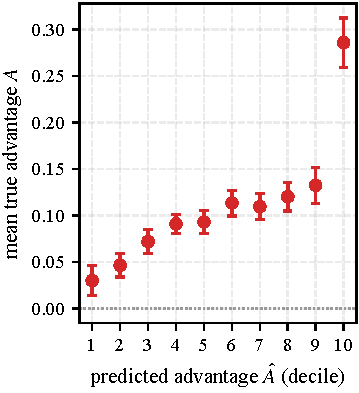
\includegraphics[width=\linewidth]{fig_calibration_kitti.pdf}\\[4pt]
{\small (a) KITTI}
\end{minipage}\hfill
%
\begin{minipage}[b]{0.30\textwidth}
\centering
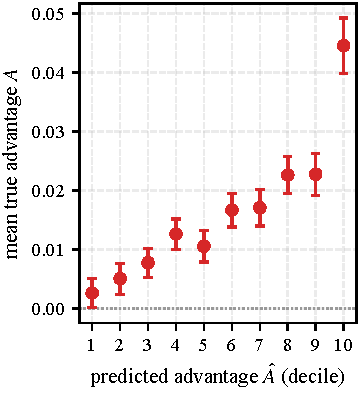
\includegraphics[width=\linewidth]{fig_calibration_bdd.pdf}\\[4pt]
{\small (b) BDD100K}
\end{minipage}\hfill
%
\begin{minipage}[b]{0.30\textwidth}
\centering
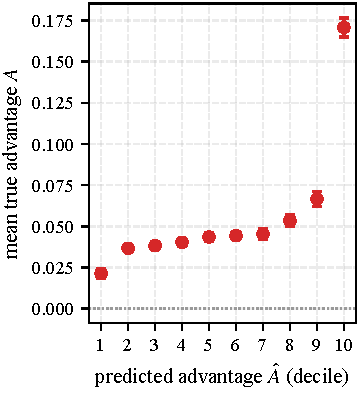
\includegraphics[width=\linewidth]{fig_calibration_waymo.pdf}\\[4pt]
{\small (c) Waymo}
\end{minipage}

\caption{
    Router ranking reliability. Validation images are grouped into deciles based on the predicted advantage $\hat{A}$ ($5$-seed ensemble).
    Each point represents the mean true advantage $A=L_{\mathrm{base}}-L_{\mathrm{super}}$ within that decile (error bars denote standard error of the mean).
    The mean true advantage increases consistently with the predicted decile across all three datasets, demonstrating that a higher router score reliably identifies frames that benefit more from the deep path.
}
\label{fig:calibration}
\end{figure*}


\begin{figure}[!t]
\centering
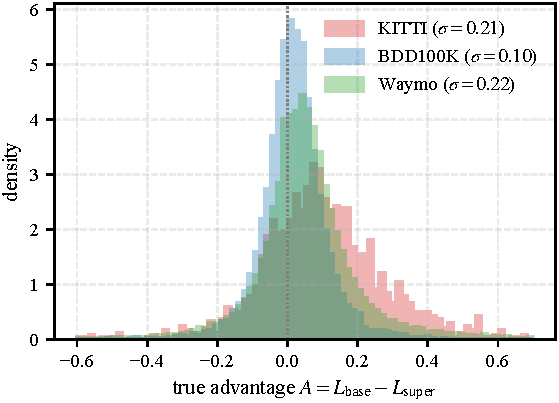
\includegraphics[width=0.9\columnwidth]{fig_advantage_dist.pdf}
\caption{Per-image advantage $A=L_{\mathrm{base}}-L_{\mathrm{super}}$ distribution on
the validation sets. Both are concentrated near zero with a long positive tail---most
frames gain little from the deep path while a minority gain a lot. The tail is wider
on KITTI ($\sigma{=}0.21$) than on BDD100K ($\sigma{=}0.10$).}
\label{fig:adv_dist}
\end{figure}

\subsubsection{Main Result}
\label{sec:results_main}

We compare the proposed advantage-regression router against the heuristic routing baselines. 
Figure~\ref{fig:main} shows that a single trained router traces a continuous Pareto frontier that consistently dominates all baselines across all three benchmarks.
In particular, the advantage of the proposed routing strategy is most pronounced in the low-budget regime, where selecting the right subset of frames for deeper execution is critical.

Table~\ref{tab:main} provides the corresponding operating points along the Pareto curve. 
On KITTI (Figure~\ref{fig:main}(a)), the router maintains AP@[.50:.95] within 0.1 point of the SUPER-only ceiling (41.4 vs.\ 41.5) while routing only 67\% of frames through the SUPER path. 
This reduces computation from 26.30 to 23.20 GFLOPs/frame ($-11.8\%$), latency from 20.69 to 18.66 ms ($-9.8\%$), and energy consumption from 3277 to 2957 mJ ($-9.8\%$), while increasing throughput from 48.3 to 53.6 FPS ($+11.0\%$). 
% A more aggressive operating point routes only 43\% of frames to the SUPER path, incurring merely a 0.3 AP reduction while lowering computation by 20.6\%, latency by 18.6\%, and energy by 18.5\%.

The same trend holds on BDD100K (Figure~\ref{fig:main}(b)).
At 55.3\% SUPER usage, the router recovers nearly all of the SUPER-path accuracy gain (22.3 vs.\ 22.5 AP@[.50:.95]) while reducing computation from 51.72 to 43.43 GFLOPs/frame ($-16.0\%$), latency from 40.06 to 33.80 ms ($-15.6\%$), and energy consumption from 13250 to 11043 mJ ($-16.7\%$).
Throughput correspondingly increases from 25.0 to 29.6 FPS ($+18.4\%$).

The same behavior carries over to the large-scale, high-resolution Waymo Open benchmark (Figure~\ref{fig:main}(c)).
At only 35\% SUPER usage, the router recovers nearly all of the SUPER-path accuracy gain (38.7 vs.\ 38.9 AP@[.50:.95], within 0.2 point of the ceiling) while reducing computation from 134.84 to 103.21 GFLOPs/frame ($-23.5\%$), latency from 16.51 to 14.05 ms ($-14.9\%$), and energy consumption from 2108 to 1677 mJ ($-20.4\%$).
Throughput correspondingly increases from 60.6 to 71.2 FPS ($+17.5\%$).
Notably, the advantage-regression router remains the only strategy that improves monotonically from the very first frames routed to the deep path, whereas the heuristic baselines (most visibly edge density) initially degrade accuracy below the always-base anchor by spending the SUPER budget on uninformative frames.

\begin{figure*}[t]
\centering
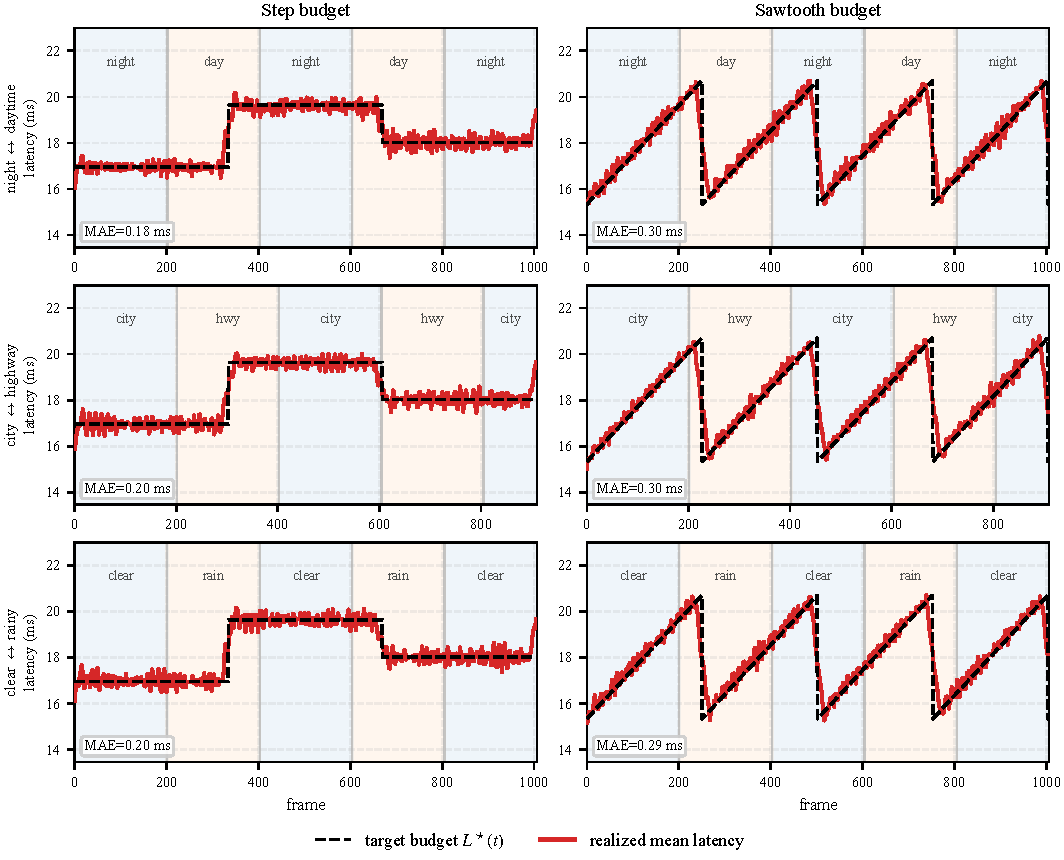
\includegraphics[width=0.85\linewidth]{fig_scenario_budget.pdf}
\caption{
    Runtime latency-budget tracking under realistic scene-condition drift on
    BDD100K MOT, run as a live on-device closed loop.
    Sequences are concatenated in alternating condition order (night$\leftrightarrow$daytime, city$\leftrightarrow$highway, clear$\leftrightarrow$rainy; rows), with shaded bands marking each segment's condition. 
    A PI controller adjusts the router threshold $\tau$ to hold a step (left)
    and a sawtooth (right) latency budget $L^\star(t)$ (black dashed); the realized mean
    latency (red) tracks it with MAE $0.18$--$0.30$\,ms across all condition drifts.
}
\label{fig:budget}
\end{figure*}


\subsubsection{Advantage Regression Quality}
\label{sec:results_calibration}

Because deployment routes by thresholding the predicted advantage $\hat{A}$, the router need not predict the exact advantage magnitude; instead, it must correctly \textit{rank} frames according to how much they benefit from the deep path. 
Figure~\ref{fig:calibration} evaluates this property by grouping validation images into deciles based on $\hat{A}$ and reporting the mean true advantage $A = L_{\text{base}} - L_{\text{super}}$ within each group. 
On all three datasets, the mean true advantage increases consistently with the predicted decile, indicating that frames assigned higher scores indeed benefit more from deeper execution.
This confirms that the router successfully captures the relative utility of the deep path, which is the key requirement for threshold-based routing. 
We emphasize ranking rather than per-image regression accuracy because the single-image target is inherently noisy, making robust ordering a more meaningful indicator of deployment performance.

The pronounced increase in the highest decile is a direct consequence of the true advantage's right-skewed distribution (Figure~\ref{fig:adv_dist}). 
While this rightward skew indicates that deeper execution generally yields lower detection losses, the distribution is heavily concentrated near zero. 
This means that for the vast majority of frames, the benefit of the super path is present but modest. 
In contrast, the long positive tail reveals that a small minority of frames experience substantial gains. 
The router successfully isolates these rare, high-payoff frames into the top-ranked decile, ensuring that limited computational resources are allocated precisely where deeper execution yields the greatest return. 
This positive tail is noticeably wider on KITTI ($\sigma{=}0.21$) and Waymo ($\sigma{=}0.22$) compared to BDD100K ($\sigma{=}0.10$). 
Accordingly, the advantage distribution on BDD100K spans a much narrower range, as reflected by the different y-axis scales in Figure~\ref{fig:calibration}, meaning that most achievable operating points for this dataset are governed by a relatively narrow band of threshold values $\tau$.


\subsubsection{Runtime Latency-Budget Tracking}
\label{sec:results_budget}
The single-scalar threshold $\tau$ exposes the operating point as a tunable dial, allowing the detector to be steered at runtime to track a time-varying latency budget $L^\star(t)$ (e.g., a thermal- or battery-driven schedule) without any retraining. 
We wrap $\tau$ in a proportional-integral (PI) control loop: the controller compares the target budget against an exponential moving average (EMA) of the realized per-frame latency and nudges $\tau$ to cancel the error. 
To stress the controller under realistic non-stationary conditions rather than abrupt synthetic boundaries, we concatenate BDD100K MOT sequences with alternating scene conditions (night$\leftrightarrow$daytime, city$\leftrightarrow$highway, clear$\leftrightarrow$rainy). 
This forces the input distribution---and hence the expected advantage of the deep path---to drift continuously as the scene evolves.

Because routing decisions are binary, each frame executes either the SUPER or BASE path, making fine-grained latency control impossible at the per-frame level. 
In practice, however, deployment constraints are typically imposed on average latency rather than individual frames. 
We therefore regulate the mean latency by adjusting the fraction of frames routed to the SUPER path through a PI controller driven by the EMA tracking error.
Figure~\ref{fig:budget} evaluates this runtime tracking in a live on-device closed loop. 
To visualize the tracked mean without the phase delay introduced by causal trailing filters, we smooth the binary per-frame latency measurements using a zero-phase (centered) moving average. 
This offline visualization preserves the true tracking behavior while avoiding smoothing-induced lag, leaving the underlying control loop unchanged.
The realized mean latency closely tracks both step and sawtooth target budgets across all condition drifts, achieving a mean absolute error of only $0.18$--$0.30$,ms. 
Ultimately, a single trained router transforms a static Pareto front into a runtime-adjustable system, enabling precise latency-budget tracking despite relying on binary per-frame routing decisions.


\subsubsection{TensorRT Deployment}
\label{sec:results_trt}
A natural concern is whether depth routing remains practical on a production inference stack: TensorRT compiles a \emph{static} graph and cannot conditionally skip layers inside a single engine.
We therefore realize routing by exporting the BASE and SUPER paths as two separate FP16 engines and keeping both resident in GPU memory; the router simply selects which engine to execute per frame.
The only routing-specific concern is then the cost of \emph{switching} between the two resident engines every time the chosen path changes.
We isolate this cost on an embedded NVIDIA Jetson Orin Nano by comparing each single-path engine run against an alternating schedule that forces a BASE$\leftrightarrow$SUPER engine switch on \emph{every} frame---a pathological worst case far more frequent than any realistic routing trace, in which the chosen path typically persists for many consecutive frames.
The switching overhead is then isolated as the latency of the alternating schedule minus the mean of the two static single-path runs.
To verify that this holds across compute scales, we report it at two input resolutions---$384\times1248$ and $736\times1280$ (the KITTI and BDD100K evaluation resolutions, respectively)---since it is the input resolution, not the dataset, that sets the per-engine cost (Table~\ref{tab:trt}).
Even under this per-frame worst case, switching costs only $+0.05\%$ at $384\times1248$ and $+0.16\%$ at $736\times1280$ over the single-path mean, confirming that engine switching is effectively free: because both FP16 engines are held resident in GPU memory, a switch merely selects which execution context to launch and incurs no weight reload or memory transfer.

Keeping all three engines (BASE, SUPER, and the router) co-resident is cheap on the embedded budget.
At the higher $736\times1280$ resolution the full routed deployment occupies $214$\,MB of GPU memory---$33$\,MB of FP16 engine weights plus $181$\,MB of activation scratch---of which the advantage-regression router is a negligible $1.3$\,MB; this is under $3\%$ of the Orin Nano's $8$\,GB.
The weights are resolution-independent (they are the detector parameters), whereas the activation scratch scales with input resolution, dropping to $97$\,MB total ($130$\,MB including weights) at $384\times1248$.
The router head adds essentially nothing, since it consumes only the small grid-pooled feature taps the detector already produces.

One deployment caveat concerns the operating threshold itself.
FP16 quantization slightly perturbs the router's predicted advantage $\hat{A}$, so a threshold $\tau$ calibrated in FP32 realizes a different SUPER usage once the engines run in FP16 (e.g., on BDD100K, $\tau{=}0.086$ routes $14.8\%$ of frames to the deep path in FP32 but $5.9\%$ in FP16).
Crucially, quantization shifts only the \emph{calibration} of $\tau$, not the ranking it induces: $\hat{A}$ remains monotone, so the same accuracy--efficiency frontier is reachable, merely at different threshold values.
Recovering a target operating point therefore requires no retraining---only a one-pass recalibration of the $\tau$-to-budget map on a small held-out clip evaluated through the FP16 engines.
In the budget-tracking deployment (Sec.~\ref{sec:results_budget}) even this step is unnecessary: the PI controller adjusts $\tau$ online from the realized latency, absorbing the FP16 shift automatically.


\begin{table}[!t]
\caption{
    TensorRT FP16 engine-switching overhead on the embedded Jetson Orin Nano (pure GPU inference, CUDA-event timed, $1000$ iterations after warm-up), reported at two input resolutions to span compute scales. \textsc{alternating} forces a BASE$\leftrightarrow$SUPER engine switch on every frame (per-frame worst case); at both resolutions its latency stays within $0.2\%$ of the mean of the two static single-path engines, so routing between two resident engines is effectively free. Resident GPU memory (FP16 weights $+$ activation scratch) is reported per engine; the router is negligible.
}
\label{tab:trt}
\small
\setlength{\tabcolsep}{5pt}
\centering
\begin{tabular}{lrrrr}
\toprule
Engine schedule & Lat.\,(ms) & FPS & Energy\,(mJ) & Mem\,(MB)\\
\midrule
\multicolumn{5}{l}{\emph{(a) $384\times1248$ (KITTI resolution)}}\\
\textsc{base} (always-base) & 12.74 & 78.5 & 218.7 & 61.7\\
\textsc{super} (always-super) & 21.10 & 47.4 & 381.4 & 68.3\\
\textsc{alternating} (switch/frame) & 16.93 & 59.1 & 300.4 & ---\\
mean(base,\,super) & 16.92 & --- & --- & \textbf{130.0}\\
switch overhead & \multicolumn{4}{l}{$+0.009$\,ms\ \ ($+0.05\%$)}\\
\midrule
\multicolumn{5}{l}{\emph{(b) $736\times1280$ (BDD100K resolution)}}\\
\textsc{base} (always-base) & 24.88 & 40.2 & 485.1 & 102.8\\
\textsc{super} (always-super) & 41.67 & 24.0 & 842.6 & 110.0\\
\textsc{router} & \multicolumn{3}{r}{(advantage head)} & 1.3\\
\textsc{alternating} (switch/frame) & 33.33 & 30.0 & 666.9 & ---\\
mean(base,\,super) & 33.27 & --- & --- & \textbf{214.1}\\
switch overhead & \multicolumn{4}{l}{$+0.052$\,ms\ \ ($+0.16\%$)}\\
\bottomrule
\end{tabular}
\end{table}


%% =====================================================================
\subsection{Ablation Studies}
\label{sec:ablation}
 
\subsubsection{Input Feature: Backbone vs. Neck vs. Both}
\label{sec:abl_feature}

\begin{figure}[t]
\centering
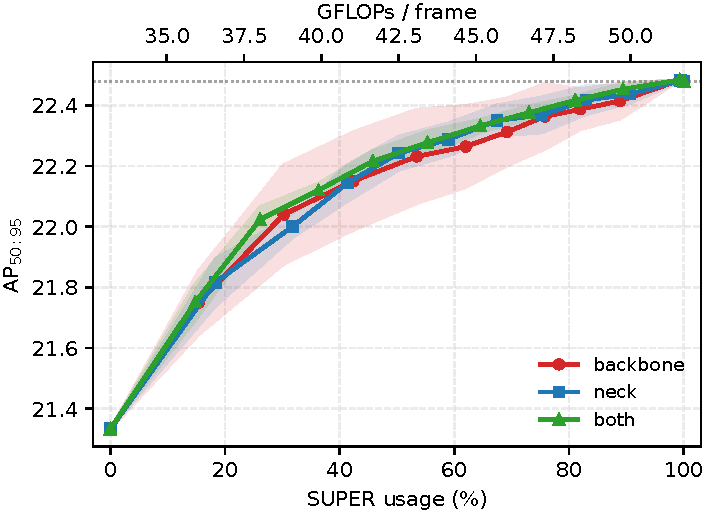
\includegraphics[width=0.9\columnwidth]{fig_abl_feat_ap5095.pdf}
\caption{
    Ablation on feature sources for the router on BDD100K. 
    Using both backbone and neck features yields the best-or-tied mean performance and the most stable routing behavior across training seeds.
}
\label{fig:abl_feat_source}
\end{figure}

We evaluate three potential feature sources for the router: the backbone pyramid features (input-level representations extracted before the detection neck), the neck features (prediction-level representations immediately preceding the detection heads), and their concatenation (both). 
Figure~\ref{fig:abl_feat_source} presents the results on BDD100K.

While all three configurations exhibit similar mean accuracy--efficiency trade-offs, their stability differs noticeably across five training seeds. 
The backbone-only router shows the widest performance variance (red shaded region). 
Because backbone features represent the visual encoding prior to multi-scale aggregation, they lack the fully fused, task-aligned context that directly dictates the final prediction difficulty. 
Relying solely on these pre-fusion features forces the router to implicitly infer the outcome of the complex neck operations, making the routing policy more sensitive to initialization and training noise.

In contrast, combining the backbone and neck features consistently achieves the best-or-tied mean performance while exhibiting the narrowest variance band. 
By providing the router with both the raw hierarchical feature state and the aggregated, task-specific context, the network observes a more comprehensive representation of the frame's inherent difficulty. 
This enables a much more robust and consistent estimation of the deep-path advantage.
Since this combined design incurs negligible additional computational overhead (Table~\ref{tab:overhead}), we adopt the \emph{both} configuration as the default feature source throughout the paper.


 
\subsubsection{Router Design and Grid Resolution}
\label{sec:abl_router}

\begin{figure}[t]
\centering
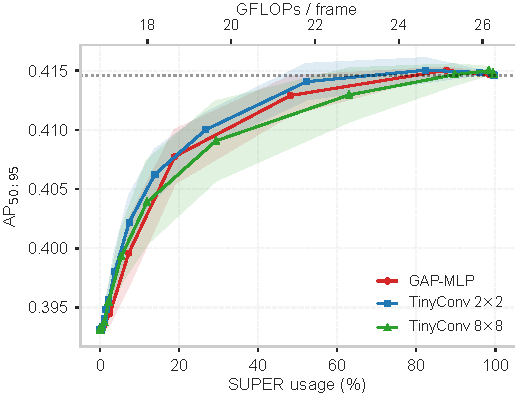
\includegraphics[width=0.9\columnwidth]{fig_abl_router_grid_ap5095.pdf}
\caption{
    Ablation on router architecture and grid resolution on KITTI. 
    % TinyConv with a coarse $2\times2$ grid consistently matches or outperforms larger grids, suggesting that preserving fine-grained spatial detail is unnecessary for robust routing decisions.
}
\label{fig:abl_router_grid}
\end{figure}

We evaluate the impact of spatial resolution on the router's predictive capacity by comparing a spatially-agnostic GAP-MLP with TinyConv architectures utilizing $2\times2$ and $8\times8$ pooling grids (Figure~\ref{fig:abl_router_grid}).
As illustrated in the performance trajectories, the TinyConv router with a coarse $2\times2$ grid consistently achieves the optimal accuracy--efficiency trade-off. 
The performance gap between the $2\times2$ variant and GAP-MLP highlights the necessity of spatial awareness. 
Because GAP-MLP globally collapses the feature maps, it entirely discards spatial layout. 
The superiority of the $2\times2$ grid demonstrates that preserving a coarse geometric context, which enables the router to roughly localize dense or difficult object clusters within the frame, provides critical cues for estimating the utility of the deep path.
Conversely, increasing the spatial grid resolution to $8\times8$ proves detrimental. 
This high-resolution configuration not only yields the lowest mean performance but also suffers from severe instability across different training seeds, as evidenced by its significantly wider variance band (green shaded area). 
This instability suggests that forcing a lightweight router to process overly fine-grained spatial details causes it to overfit to local feature noise rather than learning a robust, generalized representation of overall scene difficulty. 
Consequently, the $2\times2$ grid emerges as the optimal configuration, supplying sufficient spatial context to effectively inform routing decisions while avoiding the optimization challenges associated with higher resolutions.



\begin{figure}[t]
\centering
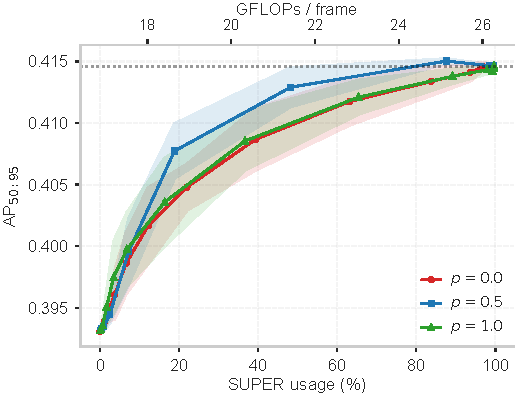
\includegraphics[width=0.9\columnwidth]{fig_abl_prevp_ap5095.pdf}
\caption{
    Ablation on the previous-action sampling ratio $p$ on KITTI. 
    The balanced setting ($p=0.5$) achieves the most robust performance by reducing train-deployment distribution shift.
}
\label{fig:abl_prevaction}
\end{figure}



\subsubsection{Previous-Action Sampling Ratio $p(\mathrm{super})$}
\label{sec:abl_prevaction}

During training, we simulate the prior frame's routing decision by sampling the assumed previous action as super with probability $p$, where $p$ represents the path whose features the router conditions on. 
We evaluate three configurations: $p \in \{0.0, 0.5, 1.0\}$. 
As illustrated Figure~\ref{fig:abl_prevaction}, the balanced setting of $p = 0.5$ yields the most robust performance, consistently outperforming both extreme configurations.
This behavior is driven by the need to mitigate train-deployment distribution shift. 
At deployment, the router must process features generated by whichever path actually executed on the previous frame. 
Since the two paths produce slightly different feature representations for the same input, training on only one path ($p=1.0$ or $p=0.0$) leaves the router poorly calibrated when the other path is encountered at runtime. 
In contrast, $p=0.5$ exposes the router equally to both feature distributions, resulting in more robust advantage estimation and more stable routing decisions during causal video inference.


